% Options for packages loaded elsewhere
% Options for packages loaded elsewhere
\PassOptionsToPackage{unicode}{hyperref}
\PassOptionsToPackage{hyphens}{url}
\PassOptionsToPackage{dvipsnames,svgnames,x11names}{xcolor}
%
\documentclass[
  super,
  preprint,
  1p,
  onecolumn]{elsarticle}
\usepackage{xcolor}
\usepackage{amsmath,amssymb}
\setcounter{secnumdepth}{5}
\usepackage{iftex}
\ifPDFTeX
  \usepackage[T1]{fontenc}
  \usepackage[utf8]{inputenc}
  \usepackage{textcomp} % provide euro and other symbols
\else % if luatex or xetex
  \usepackage{unicode-math} % this also loads fontspec
  \defaultfontfeatures{Scale=MatchLowercase}
  \defaultfontfeatures[\rmfamily]{Ligatures=TeX,Scale=1}
\fi
\usepackage{lmodern}
\ifPDFTeX\else
  % xetex/luatex font selection
\fi
% Use upquote if available, for straight quotes in verbatim environments
\IfFileExists{upquote.sty}{\usepackage{upquote}}{}
\IfFileExists{microtype.sty}{% use microtype if available
  \usepackage[]{microtype}
  \UseMicrotypeSet[protrusion]{basicmath} % disable protrusion for tt fonts
}{}
\makeatletter
\@ifundefined{KOMAClassName}{% if non-KOMA class
  \IfFileExists{parskip.sty}{%
    \usepackage{parskip}
  }{% else
    \setlength{\parindent}{0pt}
    \setlength{\parskip}{6pt plus 2pt minus 1pt}}
}{% if KOMA class
  \KOMAoptions{parskip=half}}
\makeatother
% Make \paragraph and \subparagraph free-standing
\makeatletter
\ifx\paragraph\undefined\else
  \let\oldparagraph\paragraph
  \renewcommand{\paragraph}{
    \@ifstar
      \xxxParagraphStar
      \xxxParagraphNoStar
  }
  \newcommand{\xxxParagraphStar}[1]{\oldparagraph*{#1}\mbox{}}
  \newcommand{\xxxParagraphNoStar}[1]{\oldparagraph{#1}\mbox{}}
\fi
\ifx\subparagraph\undefined\else
  \let\oldsubparagraph\subparagraph
  \renewcommand{\subparagraph}{
    \@ifstar
      \xxxSubParagraphStar
      \xxxSubParagraphNoStar
  }
  \newcommand{\xxxSubParagraphStar}[1]{\oldsubparagraph*{#1}\mbox{}}
  \newcommand{\xxxSubParagraphNoStar}[1]{\oldsubparagraph{#1}\mbox{}}
\fi
\makeatother


\usepackage{longtable,booktabs,array}
\usepackage{calc} % for calculating minipage widths
% Correct order of tables after \paragraph or \subparagraph
\usepackage{etoolbox}
\makeatletter
\patchcmd\longtable{\par}{\if@noskipsec\mbox{}\fi\par}{}{}
\makeatother
% Allow footnotes in longtable head/foot
\IfFileExists{footnotehyper.sty}{\usepackage{footnotehyper}}{\usepackage{footnote}}
\makesavenoteenv{longtable}
\usepackage{graphicx}
\makeatletter
\newsavebox\pandoc@box
\newcommand*\pandocbounded[1]{% scales image to fit in text height/width
  \sbox\pandoc@box{#1}%
  \Gscale@div\@tempa{\textheight}{\dimexpr\ht\pandoc@box+\dp\pandoc@box\relax}%
  \Gscale@div\@tempb{\linewidth}{\wd\pandoc@box}%
  \ifdim\@tempb\p@<\@tempa\p@\let\@tempa\@tempb\fi% select the smaller of both
  \ifdim\@tempa\p@<\p@\scalebox{\@tempa}{\usebox\pandoc@box}%
  \else\usebox{\pandoc@box}%
  \fi%
}
% Set default figure placement to htbp
\def\fps@figure{htbp}
\makeatother





\setlength{\emergencystretch}{3em} % prevent overfull lines

\providecommand{\tightlist}{%
  \setlength{\itemsep}{0pt}\setlength{\parskip}{0pt}}



 
\usepackage[]{natbib}
\bibliographystyle{elsarticle-num}


\usepackage{booktabs}
\usepackage{caption}
\usepackage{longtable}
\usepackage{colortbl}
\usepackage{array}
\usepackage{anyfontsize}
\usepackage{multirow}
\newpageafter{author}
\makeatletter
\@ifpackageloaded{caption}{}{\usepackage{caption}}
\AtBeginDocument{%
\ifdefined\contentsname
  \renewcommand*\contentsname{Table of contents}
\else
  \newcommand\contentsname{Table of contents}
\fi
\ifdefined\listfigurename
  \renewcommand*\listfigurename{List of Figures}
\else
  \newcommand\listfigurename{List of Figures}
\fi
\ifdefined\listtablename
  \renewcommand*\listtablename{List of Tables}
\else
  \newcommand\listtablename{List of Tables}
\fi
\ifdefined\figurename
  \renewcommand*\figurename{Figure}
\else
  \newcommand\figurename{Figure}
\fi
\ifdefined\tablename
  \renewcommand*\tablename{Table}
\else
  \newcommand\tablename{Table}
\fi
}
\@ifpackageloaded{float}{}{\usepackage{float}}
\floatstyle{ruled}
\@ifundefined{c@chapter}{\newfloat{codelisting}{h}{lop}}{\newfloat{codelisting}{h}{lop}[chapter]}
\floatname{codelisting}{Listing}
\newcommand*\listoflistings{\listof{codelisting}{List of Listings}}
\makeatother
\makeatletter
\makeatother
\makeatletter
\@ifpackageloaded{caption}{}{\usepackage{caption}}
\@ifpackageloaded{subcaption}{}{\usepackage{subcaption}}
\makeatother
\journal{The Lancet Digital Health}
\usepackage{bookmark}
\IfFileExists{xurl.sty}{\usepackage{xurl}}{} % add URL line breaks if available
\urlstyle{same}
\hypersetup{
  pdftitle={Effectiveness of a web-based intervention for individuals who committed sexual offenses against children: a concealed, prospective, parallel group, placebo-controlled, randomized trial in Germany.},
  colorlinks=true,
  linkcolor={blue},
  filecolor={Maroon},
  citecolor={Blue},
  urlcolor={Blue},
  pdfcreator={LaTeX via pandoc}}


\setlength{\parindent}{6pt}
\begin{document}

\begin{frontmatter}
\title{Effectiveness of a web-based intervention for individuals who
committed sexual offenses against children: a concealed, prospective,
parallel group, placebo-controlled, randomized trial in Germany.}
\author[1]{Peter Fromberger%
\corref{cor1}%
}
 \ead{peter.fromberger@med.uni-goettingen.de} 
\author[6]{Sonja Schröder%
%
}

\author[1]{Bruno Siegel%
%
}

\author[3]{Safiye Tozdan%
%
}

\author[2]{Andreas Leha%
%
}

\author[2]{Fabian Kück%
%
}

\author[7]{Louisa Neumann%
%
}

\author[5]{Sabine Horn%
%
}

\author[8]{Claudia Buntrock%
%
}

\author[1]{Kirsten Jordan%
%
}

\author[4]{Sonja Etzler%
%
}

\author[4]{Martin Rettenberger%
%
}

\author[5]{Anja Schiemann%
%
}

\author[3]{Peer Briken%
%
}

\author[1]{Jürgen Leo Müller%
%
}


\affiliation[1]{organization={Clinic for Psychiatry and Psychotherapy --
Forensic Psychiatry, University Medical Center
Göttingen},city={Göttingen},country={Germany},countrysep={,},postcodesep={}}
\affiliation[2]{organization={Scientific Core Facility for Medical
Biometry and Statistical Bioinformatics, University Medical Center
Göttingen},city={Göttingen},country={Germany},countrysep={,},postcodesep={}}
\affiliation[3]{organization={Institute for Sex Research, Sexual
Medicine \& Forensic Psychiatry, Center for Psychosocial Medicine,
University Medical Center
Hamburg-Eppendorf},city={Hamburg},country={Germany},countrysep={,},postcodesep={}}
\affiliation[4]{organization={Centre for
Criminology},city={Wiesbaden},country={Germany},countrysep={,},postcodesep={}}
\affiliation[5]{organization={Criminal Law, Criminal Procedure, and
Criminal Policy, University of
Cologne},city={Cologne},country={Germany},countrysep={,},postcodesep={}}
\affiliation[6]{organization={Massregelvollzugszentrum
Niedersachsen},city={Moringen},country={Germany},countrysep={,},postcodesep={}}
\affiliation[7]{organization={Clinic for Forensic Psychiatry and
Psychotherapy, KRH Psychiatry
Wunstorf},city={Wunstorf},country={Germany},countrysep={,},postcodesep={}}
\affiliation[8]{organization={Institute of Social Medicine and Health
Systems Research (ISMHSR), Otto-von-Guericke-University
Magdeburg},city={Magdeburg},country={Germany},countrysep={,},postcodesep={}}

\cortext[cor1]{Corresponding author}















        





\end{frontmatter}
    

\section*{Summary}\label{summary}

\subsection*{Background}\label{background}

Sexual offenders often present with diverse risk profiles requiring
differentiated interventions \citep{knuth84}.

\subsection*{Methods}\label{methods}

We conducted a randomized controlled trial evaluating a web-based
relapse prevention tool. The trial was prospectively registered on April
24, 2020 in the German Clinical Trial Register (DRKS00021256).

\subsection*{Findings}\label{findings}

Preliminary findings suggest significant reductions in dynamic
risk-factors.

\subsection*{Interpretations}\label{interpretations}

Taken together, the intervention did not lead to measurable changes in
the primary CARES outcome but was associated with selected improvements
in secondary endpoints --- most notably reduced explicit sexual interest
and strengthened working alliance with coaches and supervisors ---
without indications of harm also for low-risk individuals.

\subsection*{Funding}\label{funding}

The work was funded by the German Federal Ministry of Education and
Research (BMBF, Funding number: 01KR1807A). The funder of the study had
no role in study design, data collection, data analysis, data
interpretation, or writing of the report.

\begin{center}\rule{0.5\linewidth}{0.5pt}\end{center}

\newpage{}

\section*{Research in context}\label{research-in-context}
\addcontentsline{toc}{section}{Research in context}

\subsection*{Evidence before this
study}\label{evidence-before-this-study}
\addcontentsline{toc}{subsection}{Evidence before this study}

Before undertaking this study, a XXX search revealed no published
results on the efficacy of web-based intervention in reducing
risk-factors for recidivism of Individuals who committed CSA or CSEM
Offences (ICCO). The results of these reviews have been published online
2021. In summary, there existed no study reporting on the effectiveness
of WBIs. The results of a placebo-controlled randomized trial of an WBI
exclusively for CSEM users in the dark field have been reported for the
first time in 2022. The RCT demonstrated a small, but significant
reduction of time spended on viewing CSEM based on self-reports. In
2024, an updated review revealed no further empirical evidence for the
effectiveness of WBIs. More recent meta-analyses did not provide
additional empirical evdience for WBIs. To the best of our knowledge, at
the moment there is no evidence for the effectiveness of WBIS in
reducing re-offenses of CSA and CSEM.

\subsection*{Added value of this study}\label{added-value-of-this-study}
\addcontentsline{toc}{subsection}{Added value of this study}

The study provides for the first time data on the effectiveness of a WBI
for individuals who have already committed CSA or CSEM offences. While
the main outcome revealed no superiority of the WBI against a placebo
condition, secondary outcomes provide hints for superiority of the
intervention arm in reducing sexual interest. The WBI significantly
enhanced the therapeutic alliance with online coaches and community
supervisors only in the intervention arm. Adverse events were low as
well as re-offenses during trial participation.

\subsection*{Implications of all the available
evidence}\label{implications-of-all-the-available-evidence}
\addcontentsline{toc}{subsection}{Implications of all the available
evidence}

Authors should state the implications for practice or policy and future
research of their study combined with existing evidence.

\newpage{}

\section{Introduction}\label{introduction}

Child Sexual Abuse (CSA) constitutes one of the most severe adverse
experiences in child development.
\citep{piolantiGlobalPrevalenceSexual2025} The creation, sharing, and
viewing of Child Sexual Exploitation Material (CSEM) increased
significantly in the last years
\citep{baskurtMetaanalysisRecidivismRates2024}. Beyond its profound
short- and long-term consequences for survivors, CSA represents a
substantial challenge for society due to high economical costs
\citep{kewleyPreventingChildSexual2023}. These figures clearly
demonstrate the importance of preventing CSA and CSEM.

In CSA and CSEM prevention, a distinction is commonly drawn between
primary, secondary, and tertiary prevention programs. Primary prevention
initiatives are directed at children and their parents, whereas
secondary prevention programs seek to engage adults identified as being
at risk for sexual child offenses, but have not yet been convicted.
Tertiary programs have the longest history and are designed for
Individuals who already committed CSA or CSEM Offenses (ICCO).
\citep{kewleyPreventingChildSexual2023} In recent years, more and more
secondary prevention programs for ICCO have been implemented.
\citep{setoEvaluatingChildSexual2024} However, a recent meta-analysis
identified only five publications exploring the effectiveness of
secondary prevention for ICCO, none of them with a methodological high
quality.
\citep{kewleyPreventingChildSexual2023, setoEvaluatingChildSexual2024}
Thus, currently it is not possible to draw meaningful conclusions on the
effectiveness of secondary treatment programs.
\citep{setoEvaluatingChildSexual2024} The effectiveness of tertiary
treatment programs for ICCO has been studied more extensively. In a
recent meta-meta analysis, including 21 meta-analyses on tertiary
treatment programs, a overall treatment effect with an odds ratio (OR)
of 0·67 was reported. \citep{olverSexualOffenseTreatment2025} Several
moderators have been identified: community treatment programs provide
higher effect-sizes than institutional programs, individualized programs
show higher effect-sizes than group programs, high-intensity programs
are more effective than low-intensity programs, and the higher the
methodological quality, the lower the effect sizes.
\citep{holperModeratorsSexualRecidivism2024, olverSexualOffenseTreatment2025}
Up to now, most of the meta-analyses report on tertiary programs for
individuals who have been convicted for CSA. The figure for CSEM is not
as well studied. A recent review demonstrated preliminary support for
the effectiveness of these programs, but also shed light on the
methodological weakness of existing studies on the effectiveness of
prevention programs for individuals who have used CSEM: mostly, they
suffer from small sample sizes, too short follow-up periods and a lack
of officially registered re-offenses as outcome measure.
\citep{gouveiaSystematicReviewEffectiveness2025} To sum up, there exists
a broad empirical basis for a small but significant effectsize in
reducing recidivism by tertiary programs. For individuals who have been
sentenced for CSEM as well as for secondary prevention programs, the
empirical proof of effectiveness is still pending.

Originating from only having few possibilities of community-based
treatment offers (e.g.~the majority of outpatient therapists working in
the primary healthcare system are unwilling to provide treatment) and a
rising number of CSEM offenders, there exists a post-release care gap
for ICCO .
\citep{schmidtOutpatientTherapistsPerspectives2022, baskurtMetaanalysisRecidivismRates2024}
WBIs are assumed to provide greater accessibility for individuals who
face challenges in availing mental health services.
\citep{crocamoDigitalHealthInterventions2025} Thus, it was assumed that
WBIs may bridge the gap in the care of ICCO, but empirical evaluations
are scarce.
\citep{wildWebBasedHealthServices2019, hillertWebBasedInitiativesPrevent2024, schroderWebBasedInterventionsIndividuals2023}
Schröder et al.~identified six WBIs implemented in secondary prevention
without published data on their effectiveness.
\citep{schroderWebBasedInterventionsIndividuals2023} Up to now, only one
WBI (Prevent It \citep{latthEffectsInternetdeliveredCognitive2022})
reported on it's effectiveness. The authors evaluated a guided WBI on a
sample of 160 individuals who viewed more than five hours weekly CSEM at
baseline \citep{latthChildSexualAbuse2025} The Randomized Controlled
Trial (RCT) showed, that, compared with a psychological placebo,
participants of the intervention arm reported a significant, but small
decrease in weekly viewing of CSEM (Cohen's d 0·18). Besides a high
dropout rate, this study provides first evidence for the effectiveness
of WBIs for secondary prevention of individuals viewing CSEM. Only a
minority of the sample reported prior convictions (6.9\%).
\citep{hillertWebBasedInitiativesPrevent2024, setoEvaluatingChildSexual2024}
Data on an updated version are not presented yet.
\citep{haubrockCriminalPolicePerceptions} Thus, for ICCO, to the best of
our knowledge, there exist no proofed WBI yet.

\subsection{Aim of the study}\label{aim-of-the-study}

The study aimed to evaluate the effectiveness of a newly developed WBI
@myTabu for ICCO compared to a psychological placebo in a RCT. The
primary hypothesis assumes a significant reduction of dynamic
risk-factors from baseline to inter-, and post-treatment, compared to a
placebo arm. It was further assumed, that each online module within the
intervention arm will reduce the dynamic risk-factors targeted in this
module in a statistically significant manner.

\section{Method}\label{method}

\subsection{Study design and
participants}\label{study-design-and-participants}

The trial was conducted online in Germany and follows a concealed,
prospective, parallel group, placebo-control trial with 1:1
randomization. The study design has been prospectively published.
\citep{frombergerMyTabuAPlaceboControlled2021} The trial was
prospectively registered on April 24, 2020 in the
\href{https://drks.de/search/en/trial/DRKS00021256}{German Clinical
Trial Register (DRKS00021256)}. The research project was advised by a
multidisciplinary team including a representative of participants. All
individuals under community supervision (CS; §§56, 57, 68 StGB) from all
German federal states (except Hamburg, Bremen, and Saarland), which are
sentenced for at least one case of CSA (§§176ff StGB) or CSEM (§184b
StGB), were eligible. Exclusion criteria were younger than age of 18
years, a probation period shorter than six months, no access to online
intervention, a severe acute psychiatric or cerebro-organic disorder, or
a severe cognitive impairment. All participants gave written informed
consent. The participants were credited with monetary compensation
(€120). However, the participants did not receive any confirmation of
having met the treatment requirements set by court . Ethics approval was
granted by the medical ethical board of the University Medical Center
Göttingen, Göttingen, Germany, on February 21, 2020 (reference number
16/2/20).

\subsection{Randomisation and masking}\label{randomisation-and-masking}

The trial comprises two parallel arms (intervention arm and placebo
arm). Subjects are randomly allocated to treatment using an allocation
ratio of 1:1. The randomization lists are centrally generated using a
computerized system (secuTrial®, interActive Systems GmbH, Germany),
stratified by the offense type (§176ff StGB vs.~§184b StGB), type of CS,
external treatment as ordered by court, and static risk to re-offend at
baseline (assessed with the modified Static-99
\citep{setoOnlineSolicitationOffenders2012}). At screening, each subject
receives the next consecutive screening number. At randomization, each
subject eligible for study participation receives the next consecutive
randomization number according to his stratum from a block of
randomization numbers (block size: 4). Due to security reasons, blinding
of Supervison Officers (SOs) and Study Therapists (STs) was not
possible. Nevertheless, participants, outcome adjudicators, and data
analysts were blinded until the end of the data analysis.

\subsection{Procedures}\label{procedures}

The concept of the WBI framework, theoretical foundation, and content of
the WBI are published online
\citep{frombergerMyTabuAPlaceboControlled2021} and shown in the appendix
Section 2 and Figure 1. The content of the trial arms are summarized in
Table~\ref{tbl-module-content}. The WBI builds on already established
in-face community-based treatment programs following a
cognitive-behavioral approach.
\citep{brikenPraeventionSexuellenKindesmissbrauchs2017, wildPreventionSexualChild2020}
The intervention arm focus solely on psychological meaningful
risk-factors. \citep{setoEmpiricallybasedDynamicRisk2023}

\newpage{}

\begin{longtable}[]{@{}
  >{\raggedright\arraybackslash}p{(\linewidth - 4\tabcolsep) * \real{0.2500}}
  >{\raggedright\arraybackslash}p{(\linewidth - 4\tabcolsep) * \real{0.4167}}
  >{\raggedright\arraybackslash}p{(\linewidth - 4\tabcolsep) * \real{0.3333}}@{}}
\caption{Detailed description of the WBI
content.}\label{tbl-module-content}\tabularnewline
\toprule\noalign{}
\begin{minipage}[b]{\linewidth}\raggedright
Module
\end{minipage} & \begin{minipage}[b]{\linewidth}\raggedright
Intervention Content
\end{minipage} & \begin{minipage}[b]{\linewidth}\raggedright
Placebo Content
\end{minipage} \\
\midrule\noalign{}
\endfirsthead
\toprule\noalign{}
\begin{minipage}[b]{\linewidth}\raggedright
Module
\end{minipage} & \begin{minipage}[b]{\linewidth}\raggedright
Intervention Content
\end{minipage} & \begin{minipage}[b]{\linewidth}\raggedright
Placebo Content
\end{minipage} \\
\midrule\noalign{}
\endhead
\bottomrule\noalign{}
\endlastfoot
\textbf{Module 1} & • Identification of personal values and long‑term
goals to enhance treatment readiness.• Structured decision‑making and
goal‑setting to prioritize long‑term outcomes over immediate rewards. &
• Psychoeducation on benefits of physical activity and reduction of
sedentary behavior.• Goal‑setting to increase motivation and support
sustainable active lifestyles. \\
\textbf{Module 2} & • Development of collaborative skills to improve
engagement and adherence within community supervision.•
Cognitive‑behavioral strategies addressing trauma‑related avoidance and
relational functioning. & • Education on muscle function and physical
capabilities.• Identification of motivational factors and social
influences on training behavior. \\
\textbf{Module 3} & • Linking emotions to unmet needs to reduce
impulsive responding.• Mindfulness‑based strategies to improve emotional
awareness and self‑regulation. & • Education on sleep quality, stress,
and emotional regulation.• Training in behavioral strategies to
stabilize sleep routines. \\
\textbf{Module 4} & • Structured problem‑solving training to address
self‑regulation deficits.• Case‑based application to improve
decision‑making and solution evaluation. & • Education on dream
physiology and stress‑related sleep disruption.• Reflective exercises
linking sleep, stress, and executive functioning. \\
\textbf{Module 5} & • Identification and restructuring of
offense‑supportive cognitive distortions.• Case‑based illustration of
consequences of distorted thinking.• Need principle: choose three out of
16 pre-defined cognitions & • Education on nutrition and the mind--body
connection.• Practical skills to support sustainable dietary change.•
adaptive: learn more on three out of six pre-defined nutrion types \\
\textbf{Module 6} & • Differentiation of problematic and healthy sexual
interests.• Cognitive and behavioral strategies to manage high‑risk
triggers. & • Conceptualization of psychological well‑being beyond
happiness.• Self‑care practices linking nutrition, bodily awareness, and
mental stability. \\
\end{longtable}

\newpage{}

For the recruitment, scientific staff informed SOs about the trial and
asked to inform individuals under their supervision. If interested, a
meeting with an research assistant (RA) took place at the supervision
office. After obtaining the written informed consent, the RA extracted
data from official records on site. The WBI was divided into six
modules, each module was further divided into four sessions.
Participants were advised to walk through one session per week and
finish one module in one month. The next session becomes unlocked, when
one week has past and all guided exercises have been successfully
completed. User tests before running the trial took approximately 60
minutes to complete one session. All endpoints were provided online (see
appendix Table 1). Due to ethical reasons, before presenting the
questionnaire forms for the primary outcome and the Mood and Risk
Questionnaire (MRQ), participants were informed that these answers will
be viewable by their SO. To exclude a participant, the SO had to fill in
a questionnaire on exclusion reasons (Exclusion Questionnaire, EQ).
There was no time constraint defined at which a participant was
excluded. Due to data security, the trial staff had no possibility to
contact a participant directly. Communication between STs and
participants took place online. STs (one male psychotherapist, four
female psychologists) were intensively trained by completing a practice
online treatment of at least one simulated participant. Regular monthly
group supervisions ensured treatment consistency; the answers of STs on
guided exercises were manualized (appendix Figure 2). To minimize
therapist-related effects, the same STs supported both trial arms.

\subsection{Outcomes}\label{outcomes}

References, psychometric criteria and descriptions for all outcomes are
provided in the appendix Section 3. The Statistical Analysis Plan (SAP),
defines officially recorded re-offenses five years after
last-patient-out (at September 2030) and the Index of Desistance (IoD)
as primary endpoints. \citep{frombergerMyTabuAPlaceboControlled2021}
However, recently, the items of the scales underlying the IoD have been
reduced and one scale was removed due to low internal consistency; the
IoD was renamed into Child Sexual Abuse Risk Evaluation Self-Report
(CARES). The CARES is a composite measure with higher scores indicating
greater severity of both acute and stable dynamic risk-factors.
\citep{sonjaetzlerDevelopmentInitialValidationsubmitted} We report the
validated CARES (see appendix section 6.2 for pre-specified IoD).

Secondary endpoints include specific questionnaires operationalizing
these risk-factors that are thematically addressed in the individual
modules (appendix Table ??).

Frequencies of re-offenses as reported by SOs were assessed with the EQ.
Frequencies of critical events as reported by STs were assessed
continuous (appendix Figure 4), adverse events with the Mood and Risk
Questionnaire (MRQ), post-hoc defined as the occurrence of at least one
report of the highest possible score on a sub-scale.

The Working Alliance Inventory-Short Revised (WAI-SR) was used to assess
therapeutic alliance with STs and SOs. Changes in psychological
well-being have been assessed with the WHO-5 Well-Being Index (WHO-5).
To assess a possible volunteer-effect, the Questionnaire of
Non-Participation (QNP) was developed. The Questionnaire for Acceptance
of Technology (ATQ) and the Questionnaire of Subjective Therapy
Preconditions (SBV-R) were administered, but not related to the
hypotheses and not reported here. Preliminary ATQ data from the
intermediate analysis are published.
\citep{schroderAcceptanceWebBasedIntervention2024, schroderEngagementWebbasedIntervention2025}

\subsection{Statistical analysis}\label{statistical-analysis}

Data analysis was performed using the software R.
\citep{rcoreteamLanguageEnvironmentStatistical2025} Interim analysis was
done by a independent data safety monitoring board (DSMB) on April 20,
2022. Stopping guidelines have been prospectively defined (appendix
Section 1).

We found no published WBI for ICCO to guide power calculation, and
conservatively assumed small effects . Power analysis revealed a minimum
of 214 participants in each arm to be able to detect small effects (d =
0·27) with a power of 80\% at a significance level \(\alpha\) = 5\%.

Time participants needed to finish the WBI (the time from beginning of
module one to the end of the module) and working time ( the time, a
participant was working on the content of a module) was analyzed by
means of Gaussian linear model for repeated measures (MMRM) with
treatment group, time (six time-points), and treatment-by-time
interaction.

Statistical analysis for the primary outcome follows the
intention-to-treat principle (ITT). The ITT population was defined as
all participants who have completed at least one module. The CARES was
analyzed by MMRM with treatment group, time (six time-points),
treatment-by-time interaction, and the randomization strata as factors,
baseline measurements of the outcome, and the CARES as dependent
variable. Exploratively, time span from baseline was additionally added
to the MMRM as factor. A sensitivity analysis on imputed values
complemented the analysis. Imputation was done using multiple reference
based imputation followed by ANCOVA models.
\citep{wolbersStandardReferencebasedConditional2022} Non-parametric
Brunner-Munzel test for paired data (NBMP
\citep{brunnerNonparametricBehrensFisherProblem2000}) were used to
compare the pre- and post-module scores within each trial arm.
Differences from baseline were compared between trial arms using the
Non-parametric Brunner-Munzel test for unpaired data (NBMU
\citep{brunnerNonparametricBehrensFisherProblem2000}). If
discontinuation from study was due to recidivism, the participant
receives the maximal value for the remaining measurements.

To analyze the effects of each individual module, secondary endpoints
were analyzed using the NBMP comparing the pre- and post-module scores
within each trial arm. Additionally, differences from baseline were
compared between the trial arms using NBMU. Secondary endpoints were
further analyzed by fitting linear models with trial arm and
randomization strata, and pre module scores as factors and post module
scores as dependent variable. If the assumptions of a linear model were
not fulfilled either an ordinal regression model was fitted analogously
instead or the score was dichotomized in order to fit a logistic
regression model analogously. Analyses on secondary endpoints were
carried out on all participants who provided pre- and post data for the
respective module.

Frequencies and percentages of occurrences of re-offenses as reported by
the SOs and of self-reported adverse events were compared using Fisher's
exact tests. Ancilliary outcomes were not pre-sepecified. The WHO-5 was
analyzed by MMRM with treatment group, time (six time-points),
treatment-by-time interaction, and the randomization strata as factors,
baseline measurements of the outcome and the WHO-5 as dependent
variable. The same analysis rationale was applied for the WAI-SR COACH
and WAI-SR SUPERVISOR with five time-points.

The error terms of all MMRMs were assumed to follow a multivariate
normal distribution with unstructured covariance. Least squares mean
changes from baseline are reported for the trial arms with 95\%
confidence interval (CI) as well as the difference between the least
squares treatment group means with 95\% CI and p-value testing the null
hypothesis of no treatment effect. For all multiple comparisons,
p-values were adjusted using the Bonferroni-Holm's method. All tests
were performed two-sided with 5\% significance level.

\subsection{Role of funding source}\label{role-of-funding-source}

The work was funded by the BMBF (Funding number: 01KR1807A). The funder
had no role in study design, data collection, data analysis, data
interpretation, or writing of the report.

\section{Results}\label{results}

Between March 01, 2020, and Septembre 30, 2024, 385 individuals who
committed sexual offenses against children have been screened for
eligibility, of whom 16 have not been randomized (see
Figure~\ref{fig-diagram-consort-flowchart}). 369 individuals were
randomly assigned (182 placebo arm; 187 intervention arm). 213
participants have been included in the ITT sample (107 {[}57·2\%{]}
intervention arm; 106 {[}58·2\%{]} placebo arm). 99 participants
finished the WBI (44 {[}30·2\%{]} intervention arm; 55 {[}22·4\%{]}
placebo arm). The trial was closed at Septembre 30, 2024. 70
participants were not able to finish the WBI before closing (39
{[}59\%{]} intervention arm; 31 {[}53\%{]} placebo arm).

The trial profile is shown in Table~\ref{tbl-baseline-characteristics}.
Only two screened participants gave informed consent to fill in the QNP,
not allowing any inferences. Participants mean age was 41 years (range
20 to 68), predominantly male (216 {[}98\%{]}; female: 2 {[}0·9\%{]};
transsexual: 1 {[}0·5\%{]}; other: 1 {[}0·5\%{]}), and with a mean of 13
years of education (range 4 to 21 years). With regard to strata, 89
(40\%) participants were mixed offenders (at least one conviction §176ff
StG) and 132 (60\%) hands-off offenders (only convictions based on
\$184b StGB). 176 (80\%) participants were under CS (§§56, 57 StGB), 45
(20\%) under post-release supervision (§§68ff StGB). 70 participants
(32\%) received an external psychotherapy and/or medical treatment, 151
(68\%) not. The court ordered treatment for 124 (56\%), for 87 (44\%)
not. 48 (39\%) of all participants, who had an court ordered treatment,
received external treatment, 76 (61\%) not. 180 participants (81\%) had
a low to medium static recidivism risk, 41 (19\%) a medium to high
static risk to re-offend at baseline. The most common psychiatric
conditions were other depressive syndromes (20 {[}9\%{]}), and
somatoform syndromes (17 {[}7·7\%{]}). Psychosocial functioning was
generally good (130 {[}59\%{]} reporting no difficulty at all). Seven
(3·2\%) participants full-filled the diagnostic criteria for a
pedophilic disorder, 213 (97\%) not. Data on ethnicity was not assessed.

\newpage{}

\begin{figure}

\centering{

\pandocbounded{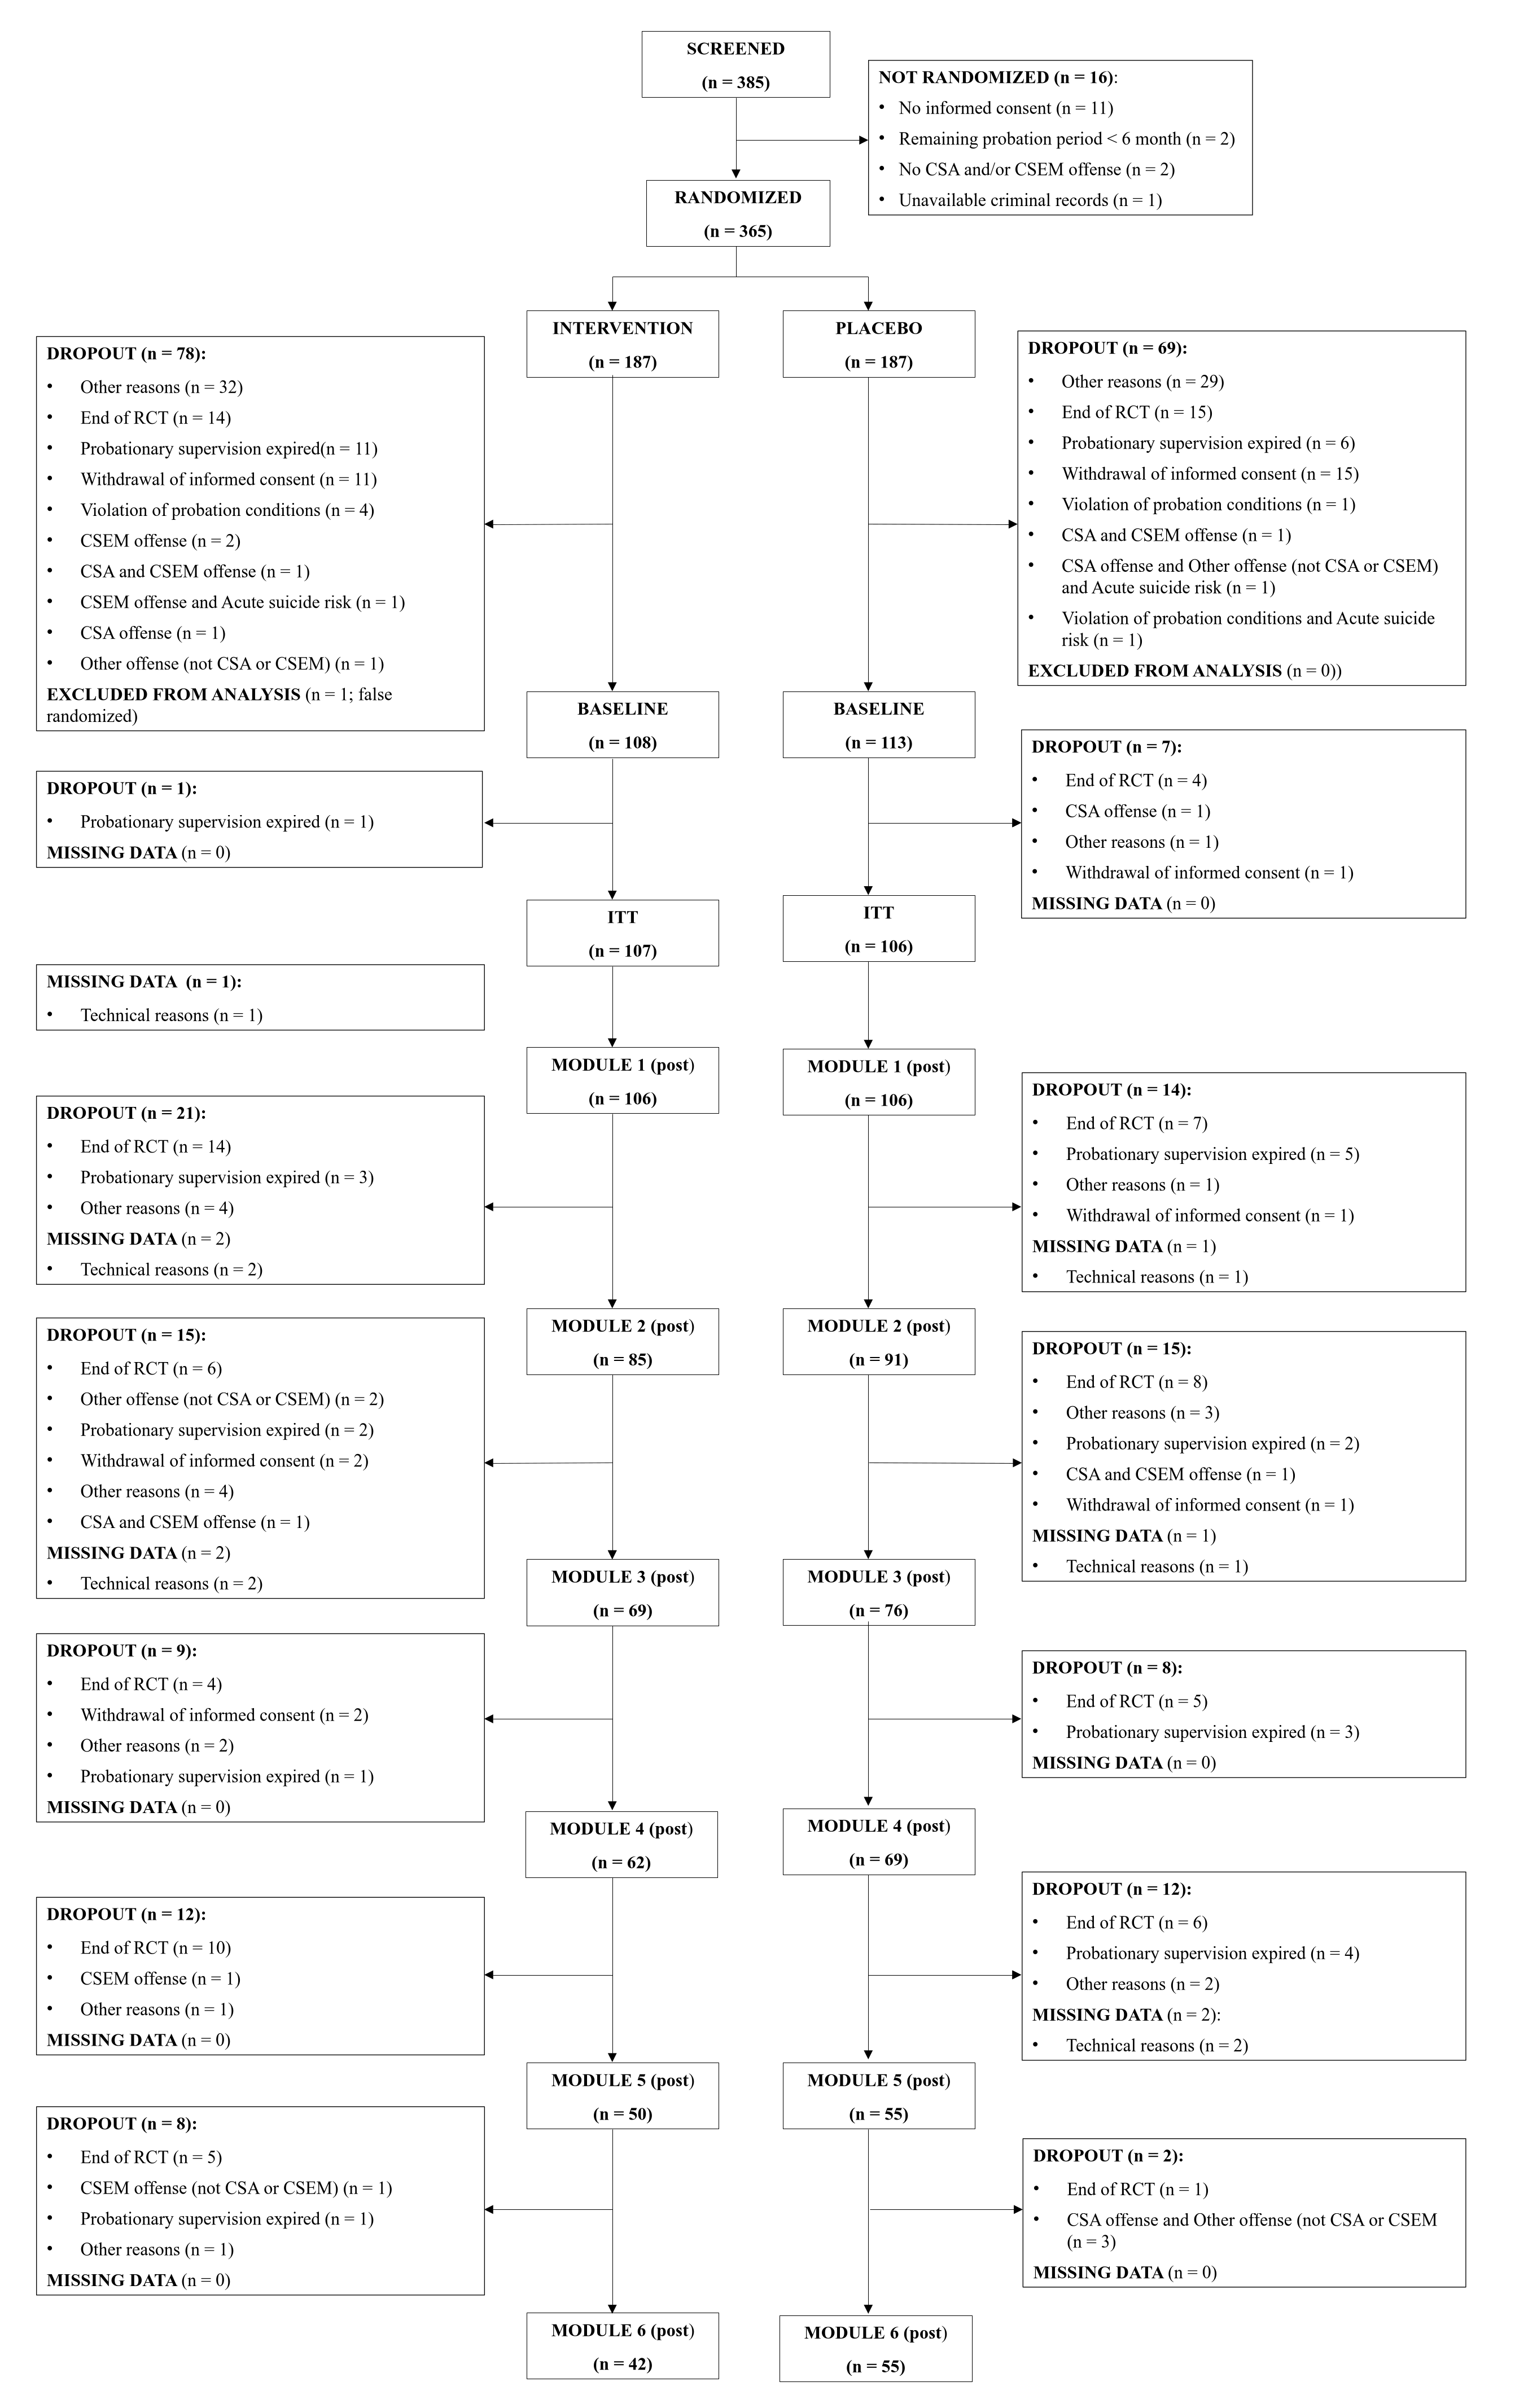
\includegraphics[keepaspectratio]{resources/diagrams/fig-trial-profile-smaller.png}}

}

\caption{\label{fig-diagram-consort-flowchart}Trial profile. ITT =
Intention-to-treat population. StGB = German penalty law.}

\end{figure}%

\newpage{}

The mixed model for repeated measures (MMRM) for the primary endpoint
showed no evidence of a treatment effect over time (all p≥0·15). Strata
as factors had no significant effect (all p≥0·13; see
Table~\ref{tbl-prim-cares-mmrm}). Sensitivity analysis (all p≥0·169;
appendix Table 8) and a MMRM additionally adjusted for time since the
beginning of module\,one revealed no significance (all p≥0·293; appendix
Table 11). Within‑arm pairwise comparisons in the intervention arm
showed a significant reduction at module\,one from median 12 (Q1 8 to Q3
18) to median 12 (Q1 6 to Q3 16, p=0·0050, p\textsubscript{adj}=0·030)
and at module 3 from median 11 (Q1 4 to Q3 17) to median 9 (Q1 5 to Q3
16, p\textless0·010, p\textsubscript{adj}=0·050; appendix Table 9). In
the placebo arm, there was a significant reduction at module 1 from
median 11 (Q1 7 to Q3 16) to median 9 (Q1 4 to Q3 16, p\textless0.0001,
p\textsubscript{adj}\textless0.0001), at module two a increase from
median 8 (Q1 4 to Q3 16) to median 10 (Q1 4 to Q3 14, p=0.050,
p\textsubscript{adj}=0.21), and a decrease at module three from median
10 (Q1 5 to Q3 18) to median 8 (Q1 5 to Q3 14, p=0.041,
p\textsubscript{adj}=0.21; appendix Table 10). Change from baseline
between trial arms showed no significant effects (all p≥0·052; appendix
Table\,11). The SAP-conform analysis of the IoD yielded no significant
effects (all p≥0·588; appendix section 6.2).

\newpage{}

\begin{table}

\caption{\label{tbl-baseline-characteristics}Baseline characteristics by
trial arm.}

\centering{

\fontsize{9.0pt}{11.0pt}\selectfont
\begin{tabular*}{\linewidth}{@{\extracolsep{\fill}}lccc}
\toprule
\textbf{Characteristic} & \textbf{Overall}  N = 221\textsuperscript{\textit{1}} & \textbf{Intervention}  N = 108\textsuperscript{\textit{1}} & \textbf{Placebo}  N = 113\textsuperscript{\textit{1}} \\ 
\midrule\addlinespace[2.5pt]
{\bfseries Age}\textsuperscript{\textit{2}} & 42 (20 - 68) & 41 (20 - 66) & 43 (21 - 68) \\ 
{\bfseries Years of education}\textsuperscript{\textit{3}} & 13 (4 - 21) & 12 (7 - 21) & 13 (4 - 20) \\ 
{\bfseries Highest education}\textsuperscript{\textit{3}} &  &  &  \\ 
    No formal education & 17 (7·7\%) & 10 (9·3\%) & 7 (6·2\%) \\ 
    Lower secondary school & 88 (40\%) & 42 (39\%) & 46 (41\%) \\ 
    Intermediate secondary school & 70 (32\%) & 36 (33\%) & 34 (30\%) \\ 
    Upper secondary school & 30 (14\%) & 13 (12\%) & 17 (15\%) \\ 
    University degree & 16 (7·2\%) & 7 (6·5\%) & 9 (8·0\%) \\ 
{\bfseries Employment status}\textsuperscript{\textit{3}} &  &  &  \\ 
    Unemployed & 61 (28\%) & 29 (27\%) & 32 (28\%) \\ 
    In education/training & 11 (5·0\%) & 6 (5·6\%) & 5 (4·4\%) \\ 
    Unskilled worker & 8 (3·6\%) & 5 (4·6\%) & 3 (2·7\%) \\ 
    Worker & 61 (28\%) & 32 (30\%) & 29 (26\%) \\ 
    Employee & 51 (23\%) & 25 (23\%) & 26 (23\%) \\ 
    Self-employed & 8 (3·6\%) & 4 (3·7\%) & 4 (3·5\%) \\ 
    Retired & 21 (9·5\%) & 7 (6·5\%) & 14 (12\%) \\ 
{\bfseries Marital status}\textsuperscript{\textit{3}} &  &  &  \\ 
    Single & 144 (65\%) & 79 (73\%) & 65 (58\%) \\ 
    Married & 44 (20\%) & 15 (14\%) & 29 (26\%) \\ 
    Divorced & 29 (13\%) & 12 (11\%) & 17 (15\%) \\ 
    Widowed & 4 (1·8\%) & 2 (1·9\%) & 2 (1·8\%) \\ 
{\bfseries Gender}\textsuperscript{\textit{4}} &  &  &  \\ 
    Female & 2 (0·9\%) & 2 (1·9\%) & 0 (0\%) \\ 
    Male & 216 (98\%) & 105 (97\%) & 111 (99\%) \\ 
    Trans/Transsexual & 1 (0·5\%) & 0 (0\%) & 1 (0·9\%) \\ 
    Other & 1 (0·5\%) & 1 (0·9\%) & 0 (0\%) \\ 
    Missing & 1 & 0 & 1 \\ 
{\bfseries Sexual orientation}\textsuperscript{\textit{4}} &  &  &  \\ 
    Exclusively heterosexual & 145 (66\%) & 72 (67\%) & 73 (65\%) \\ 
    Predominantly heterosexual & 24 (11\%) & 10 (9·3\%) & 14 (13\%) \\ 
    Bisexual & 26 (12\%) & 12 (11\%) & 14 (13\%) \\ 
    Predominantly homosexual & 3 (1·4\%) & 2 (1·9\%) & 1 (0·9\%) \\ 
    Exclusively homosexual & 11 (5·0\%) & 5 (4·6\%) & 6 (5·4\%) \\ 
    Asexual & 3 (1·4\%) & 3 (2·8\%) & 0 (0\%) \\ 
    Other & 8 (3·6\%) & 4 (3·7\%) & 4 (3·6\%) \\ 
    Missing & 1 & 0 & 1 \\ 
{\bfseries Offense type}\textsuperscript{\textit{2}} &  &  &  \\ 
    Hands-on (at least one conviction §176ff StGB) & 89 (40\%) & 44 (41\%) & 45 (40\%) \\ 
    Hands-off (only §184b StGB) & 132 (60\%) & 64 (59\%) & 68 (60\%) \\ 
{\bfseries Type of supervision}\textsuperscript{\textit{5}} &  &  &  \\ 
    post-release supervision & 45 (20\%) & 20 (19\%) & 25 (22\%) \\ 
    community supervision & 176 (80\%) & 88 (81\%) & 88 (78\%) \\ 
{\bfseries Static recidivism risk}\textsuperscript{\textit{6}} &  &  &  \\ 
    Low-medium & 180 (81\%) & 87 (81\%) & 93 (82\%) \\ 
    Medium-high risk & 41 (19\%) & 21 (19\%) & 20 (18\%) \\ 
{\bfseries Term of imprisonment (month)}\textsuperscript{\textit{7}} & 22 (0 - 156) & 21 (0 - 126) & 23 (0 - 156) \\ 
    Missing & 3 & 1 & 2 \\ 
{\bfseries Treatment ordered by court}\textsuperscript{\textit{7}} &  &  &  \\ 
    Yes & 124 (56\%) & 62 (57\%) & 62 (55\%) \\ 
    No & 97 (44\%) & 46 (43\%) & 51 (45\%) \\ 
{\bfseries Additional treatment}\textsuperscript{\textit{2}} &  &  &  \\ 
    Yes & 70 (32\%) & 33 (31\%) & 37 (33\%) \\ 
    No & 151 (68\%) & 75 (69\%) & 76 (67\%) \\ 
{\bfseries Major depressive syndrome}\textsuperscript{\textit{8}} &  &  &  \\ 
    Yes & 12 (5·4\%) & 6 (5·6\%) & 6 (5·3\%) \\ 
    No & 209 (95\%) & 102 (94\%) & 107 (95\%) \\ 
{\bfseries Other depressive syndromes}\textsuperscript{\textit{8}} &  &  &  \\ 
    Yes & 20 (9·0\%) & 12 (11\%) & 8 (7·1\%) \\ 
    No & 201 (91\%) & 96 (89\%) & 105 (93\%) \\ 
{\bfseries Panic syndrome}\textsuperscript{\textit{8}} &  &  &  \\ 
    Yes & 5 (2·3\%) & 2 (1·9\%) & 3 (2·7\%) \\ 
    No & 216 (98\%) & 106 (98\%) & 110 (97\%) \\ 
{\bfseries Other anxiety syndromes}\textsuperscript{\textit{8}} &  &  &  \\ 
    Yes & 3 (1·4\%) & 3 (2·8\%) & 0 (0\%) \\ 
    No & 218 (99\%) & 105 (97\%) & 113 (100\%) \\ 
{\bfseries Bulimia nervosa}\textsuperscript{\textit{8}} &  &  &  \\ 
    Yes & 0 (0\%) & 0 (0\%) & 0 (0\%) \\ 
    No & 221 (100\%) & 108 (100\%) & 113 (100\%) \\ 
{\bfseries Binge eating}\textsuperscript{\textit{8}} &  &  &  \\ 
    Yes & 8 (3·6\%) & 3 (2·8\%) & 5 (4·4\%) \\ 
    No & 213 (96\%) & 105 (97\%) & 108 (96\%) \\ 
{\bfseries Alcohol syndrome}\textsuperscript{\textit{8}} &  &  &  \\ 
    Yes & 11 (5·0\%) & 6 (5·6\%) & 5 (4·4\%) \\ 
    No & 210 (95\%) & 102 (94\%) & 108 (96\%) \\ 
{\bfseries Somatoform syndrome}\textsuperscript{\textit{8}} &  &  &  \\ 
    Yes & 17 (7·7\%) & 8 (7·4\%) & 9 (8·0\%) \\ 
    No & 204 (92\%) & 100 (93\%) & 104 (92\%) \\ 
{\bfseries Psychosocial functioning} &  &  &  \\ 
    Not difficult at all & 130 (59\%) & 60 (56\%) & 70 (62\%) \\ 
    Somewhat difficult & 76 (34\%) & 37 (34\%) & 39 (35\%) \\ 
    Very difficult & 13 (5·9\%) & 10 (9·3\%) & 3 (2·7\%) \\ 
    Extremely difficult & 2 (0·9\%) & 1 (0·9\%) & 1 (0·9\%) \\ 
{\bfseries 6D30 Exhibitionistic disorder}\textsuperscript{\textit{4}} &  &  &  \\ 
    Yes & 1 (0·5\%) & 1 (0·9\%) & 0 (0\%) \\ 
    No & 219 (100\%) & 107 (99\%) & 112 (100\%) \\ 
    Missing & 1 & 0 & 1 \\ 
{\bfseries 6D31 Voyeuristic disorder}\textsuperscript{\textit{4}} &  &  &  \\ 
    Yes & 5 (2·3\%) & 4 (3·7\%) & 1 (0·9\%) \\ 
    No & 215 (98\%) & 104 (96\%) & 111 (99\%) \\ 
    Missing & 1 & 0 & 1 \\ 
{\bfseries 6D32 Pedophilic disorder}\textsuperscript{\textit{4}} &  &  &  \\ 
    Yes & 7 (3·2\%) & 4 (3·7\%) & 3 (2·7\%) \\ 
    No & 213 (97\%) & 104 (96\%) & 109 (97\%) \\ 
    Missing & 1 & 0 & 1 \\ 
{\bfseries 6D33 Coercive sexual sadism disorder}\textsuperscript{\textit{4}} &  &  &  \\ 
    Yes & 2 (0·9\%) & 2 (1·9\%) & 0 (0\%) \\ 
    No & 218 (99\%) & 106 (98\%) & 112 (100\%) \\ 
    Missing & 1 & 0 & 1 \\ 
{\bfseries 6D34 Frotteuristic disorder}\textsuperscript{\textit{4}} &  &  &  \\ 
    Yes & 1 (0·5\%) & 1 (0·9\%) & 0 (0\%) \\ 
    No & 219 (100\%) & 107 (99\%) & 112 (100\%) \\ 
    Missing & 1 & 0 & 1 \\ 
{\bfseries 6D35 Other paraphilic disorder (non-consenting)}\textsuperscript{\textit{4}} &  &  &  \\ 
    Yes & 1 (0·5\%) & 1 (0·9\%) & 0 (0\%) \\ 
    No & 219 (100\%) & 107 (99\%) & 112 (100\%) \\ 
    Missing & 1 & 0 & 1 \\ 
\bottomrule
\end{tabular*}
\begin{minipage}{\linewidth}
\vspace{.05em}
\parbox{\linewidth}{\raggedright {\textsuperscript{\textit{1}} Mean (Min - Max); n (\%)}}\\
\parbox{\linewidth}{\raggedright {\textsuperscript{\textit{2}} data extracted from case files by trained staff (Sample Specifications Questionnaire based on the Court File, SSQ-CF).}}\\
\parbox{\linewidth}{\raggedright {\textsuperscript{\textit{3}} information provided by the participant (Sample Specifications Questionnaire for the Participant, SSQ-P).}}\\
\parbox{\linewidth}{\raggedright {\textsuperscript{\textit{4}} assessed with the ICD-11 screener, a self-report measure which items follow the ICD-11 diagnostic criteria for paraphilic disorders.}}\\
\parbox{\linewidth}{\raggedright {\textsuperscript{\textit{5}} information provided by supervision officer (SSQ-SO); in the German legal system, probation service refers to supervision and support during a suspended sentence or post-release support after prison, while post-release supervision (Führungsaufsicht) is a court-ordered measure of control and assistance after imprisonment in a high security hospital.}}\\
\parbox{\linewidth}{\raggedright {\textsuperscript{\textit{6}} data extracted from case files by trained staff (Sample Specifications Questionnaire based on the Court File, SSQ-CF); since the Static-99 is only defined for hands-on offenders, the reduced Static-99 as mentioned by Seto et al. (2012) was used); all staff member have been trained for the Static-99.}}\\
\parbox{\linewidth}{\raggedright {\textsuperscript{\textit{7}} information provided by supervision officer (Sample Specifications Questionnaire for the SO, SSQ-SO).}}\\
\parbox{\linewidth}{\raggedright {\textsuperscript{\textit{8}} assessed with the PHQ-D.}}\\
\parbox{\linewidth}{\raggedright {Abbreviation: ICD-11 = International Classification of Disease version 11, StGB = German penalty law.\\
}}\end{minipage}

}

\end{table}%

\newpage{}

Analysis of secondary outcomes showed for the intervention arm a
significantly decrease in ESIQ from median 87 (Q1\,80 to Q3\,98) to
median 87 (Q1\,80 to Q3\,90; p=0·0010, p\textsubscript{adj}=0·016),
indicating a reduction in sexual interests in children. The SSIC
increased from median 28 (Q1\,26 to Q3\,30) to median 30 (Q1\,25 to
Q3\,30, p\,=\,0·049, q\,=\,0·59), the CVTRQ increased from median 85
(Q1\,79 to Q3\,90) to median 87 (Q1\,80 to Q3\,92), indicating improved
treatment readiness (p=0·0060; p\textsubscript{adj}=0·078), and the DERS
increased from median 5 (Q1\,5 to Q3\,6·5) to median 6 (Q1\,5 to Q3\,8,
p=0·0050, p\textsubscript{adj}=0·070), indication detoriation of emotion
regulation. All other secondary endpoints revealed not significance (all
p\,≥\,0·066; Table~\ref{tbl-sec-pairwise-intervention}). In the placebo
arm, only the F‑Soz‑U increased from median 3·86 (Q1 3·14 to Q3 4·43) at
baseline to median 4 (Q1 3·29 to Q3 4·71) at post‑measurement (p=0·0030,
p\textsubscript{adj}=0·045), no other significant differences were
observed (all p≥0·12; Table~\ref{tbl-sec-pairwise-placebo}).

Exploratory analyses of change from baseline showed that the ESIQ
decreased in the intervention arm (median change −3, Q1 -8 to 0), but
remained largely unchanged in the placebo arm (median change 0, Q1 -1 to
Q3 0, p=0·0020, p\textsubscript{adj}=0·030). Change from baseline in the
DERS was greater in the intervention arm (median change 0, Q1 0 to 1)
than in the placebo arm (median change 0, Q1 0 to Q3 0, p=0·024,
p\textsubscript{adj}=0·34). All other secondary endpoints showed no
significant differences between trial arms (all p≥0·077; appendix Table
18). Explorative regression models fitting randomization strata as
factors support this figure (appendix Section 7).

\newpage{}

\begin{table}

\caption{\label{tbl-prim-cares-mmrm}Mixed model for repeated measures
(MMRM) for the primary endpoint Child Sexual Abuse Risk Evaluation
Self-Report (CARES total score).}

\centering{

\fontsize{9.0pt}{11.0pt}\selectfont
\begin{tabular*}{\linewidth}{@{\extracolsep{\fill}}llll}
\toprule
\textbf{Variable} & \textbf{Beta} & \textbf{95\% CI} & \textbf{p-value} \\ 
\midrule\addlinespace[2.5pt]
{\bfseries (Intercept)} & -0·34 & -1·9 to 1·2 & 0·67 \\ 
{\bfseries Type of supervision} &  &  &  \\ 
    community supervision & 0·00 & Ref. &  \\ 
    post-release supervision & 0·32 & -1·2 to 1·8 & 0·68 \\ 
{\bfseries Additional treatment} &  &  &  \\ 
    No & 0·00 & Ref. &  \\ 
    Yes & -0·92 & -2·1 to 0·27 & 0·13 \\ 
{\bfseries Offense type} &  &  &  \\ 
    Hands-off (only §184b StGB) & 0·00 & Ref. &  \\ 
    Hands-on (at least one conviction §176 ff StGB) & 0·93 & -0·29 to 2·2 & 0·13 \\ 
{\bfseries Baseline value} & 0·84 & 0·77 to 0·91 & <0·0001 \\ 
{\bfseries Static recidivism risk} & 0·38 & -0·13 to 0·88 & 0·14 \\ 
{\bfseries Timepoint * treatment} &  &  &  \\ 
    Module 1 (post) * Intervention & 0·39 & -0·83 to 1·6 & 0·53 \\ 
    Module 2 (post) * Intervention & -0·97 & -2·6 to 0·65 & 0·24 \\ 
    Module 3 (post) * Intervention & -0·33 & -1·9 to 1·3 & 0·68 \\ 
    Module 4 (post) * Intervention & -0·25 & -1·8 to 1·3 & 0·75 \\ 
    Module 5 (post) * Intervention & -0·14 & -2·0 to 1·8 & 0·89 \\ 
    Module 6 (post) * Intervention & -0·61 & -2·6 to 1·4 & 0·54 \\ 
{\bfseries Timepoint} &  &  &  \\ 
    Module 1 (post) & 0·00 & Ref. &  \\ 
    Module 2 (post) & 0·98 & -0·01 to 2·0 & 0·052 \\ 
    Module 3 (post) & -0·46 & -1·4 to 0·50 & 0·34 \\ 
    Module 4 (post) & -0·53 & -1·6 to 0·51 & 0·31 \\ 
    Module 5 (post) & 0·07 & -1·1 to 1·3 & 0·91 \\ 
    Module 6 (post) & 0·16 & -0·97 to 1·3 & 0·78 \\ 
\bottomrule
\end{tabular*}
\begin{minipage}{\linewidth}
\vspace{.05em}
\parbox{\linewidth}{\raggedright {Abbreviation: CI = Confidence Interval, StGB = German penalty law.\\
}}\end{minipage}

}

\end{table}%

\newpage{}

The MMRM for the cumulative time from baseline to finish module showed a
significant treatment-by-time interaction across all timepoints (all
p≤0·035, appendix Table 3). Post-hoc pairwise comparisons showed longer
times in the intervention arm for all modules. Unadjusted analyses
indicated significant differences at module four (mean 260 days, SD 138,
intervention arm; mean 223 days, SD 122, placebo arm; p=0·048) and
module five (mean 325 days, SD 161 intervention arm; mean 258 days, SD
113 placebo arm, p=0·028), whereas differences at modules one, two,
three, and six did not reach significance (all p≥0·053). After
adjustment for multiple comparisons, none remained significant (all
q≥0·17; appendix Table 4).

The MMRM for the time working on content revealed a significant
treatment-by-time interaction at module one (\(\beta\) 360 hours, 95\%
CI 49 to 671, p=0·024), module four (\(\beta\) 236 hours, 95\% CI 19 to
453, p=0·034), and at module five (\(\beta\) 324 hours, 95\% CI 6.1 to
641, p=0·046). No significance was observed at module two (\(\beta\) 148
hours, 95\% CI -48 to 345, p=0·14), module three (\(\beta\) 188 hours,
95\% CI -96 to 473, p=0·19), and module six (\(\beta\) 93 hours, 95\% CI
-142 to 328, p=0·42; appendix Table 5). Post-hoc pairwise comparisons
reveled no differences between trial arms (all p≥0·18; appendix Table 6)

\newpage{}

\begin{table}

\caption{\label{tbl-sec-pairwise-placebo}Pairwise comparisons between
pre- and post module scores of secondary endpoints within the placebo
arm.}

\centering{

\fontsize{9.0pt}{11.0pt}\selectfont
\begin{tabular*}{\linewidth}{@{\extracolsep{\fill}}lcccc}
\toprule
\textbf{Characteristic} & \textbf{Pre}  N = 113 & \textbf{Post}  N = 113 & \textbf{p} & \textbf{p\textsubscript{adj}} \\ 
\midrule\addlinespace[2.5pt]
{\bfseries CVTRQ (total score)} &  &  & 0·12 & >0·99 \\ 
    Mean (SD) & 85 (7) & 86 (8) &  &  \\ 
    Median (Q1, Q3) & 86 (81, 91) & 87 (81, 91) &  &  \\ 
    Min, Max & 67, 100 & 61, 100 &  &  \\ 
{\bfseries RCQ (total score)} &  &  & 0·41 & >0·99 \\ 
    Mean (SD) & 25·7 (3·8) & 26·1 (3·5) &  &  \\ 
    Median (Q1, Q3) & 26·0 (24·0, 28·0) & 26·0 (24·0, 28·0) &  &  \\ 
    Min, Max & 16·0, 38·0 & 15·0, 32·0 &  &  \\ 
{\bfseries F-Soz-U (total score)} &  &  & 0·0030 & 0·048 \\ 
    Mean (SD) & 3·74 (0·84) & 3·88 (0·89) &  &  \\ 
    Median (Q1, Q3) & 3·86 (3·14, 4·43) & 4·00 (3·29, 4·71) &  &  \\ 
    Min, Max & 1·71, 5·00 & 1·71, 5·00 &  &  \\ 
    Missing & 19 & 19 &  &  \\ 
{\bfseries OQMPR (total score)} &  &  & 0·25 & >0·99 \\ 
    Mean (SD) & 29 (7) & 28 (8) &  &  \\ 
    Median (Q1, Q3) & 29 (24, 34) & 28 (22, 33) &  &  \\ 
    Min, Max & 15, 43 & 12, 47 &  &  \\ 
    Missing & 19 & 19 &  &  \\ 
{\bfseries UCLA (total score)} &  &  & 0·51 & >0·99 \\ 
    Mean (SD) & 28·2 (3·8) & 28·1 (4·7) &  &  \\ 
    Median (Q1, Q3) & 27·0 (25·0, 30·0) & 27·0 (25·0, 31·0) &  &  \\ 
    Min, Max & 20·0, 39·0 & 12·0, 42·0 &  &  \\ 
    Missing & 19 & 19 &  &  \\ 
{\bfseries BIS-15 (total score)} &  &  & 0·96 & >0·99 \\ 
    Mean (SD) & 29 (6) & 29 (6) &  &  \\ 
    Median (Q1, Q3) & 28 (25, 32) & 28 (25, 32) &  &  \\ 
    Min, Max & 16, 50 & 17, 47 &  &  \\ 
    Missing & 35 & 35 &  &  \\ 
{\bfseries CUSI (total score)} &  &  & 0·12 & >0·99 \\ 
    Mean (SD) & 27 (8) & 28 (8) &  &  \\ 
    Median (Q1, Q3) & 26 (22, 30) & 28 (23, 32) &  &  \\ 
    Min, Max & 16, 60 & 16, 59 &  &  \\ 
    Missing & 35 & 35 &  &  \\ 
{\bfseries DERS (subscale impulsivity)} &  &  & 0·59 & >0·99 \\ 
    Mean (SD) & 6·08 (1·75) & 5·92 (1·55) &  &  \\ 
    Median (Q1, Q3) & 5·00 (5·00, 7·00) & 5·00 (5·00, 6·00) &  &  \\ 
    Min, Max & 5·00, 13·00 & 5·00, 10·00 &  &  \\ 
    Missing & 35 & 35 &  &  \\ 
{\bfseries NARQ (subscale externalizing strategies)} &  &  & 0·76 & >0·99 \\ 
    Mean (SD) & 1·88 (2·75) & 1·59 (2·12) &  &  \\ 
    Median (Q1, Q3) & 1·00 (0·00, 3·00) & 1·00 (0·00, 2·00) &  &  \\ 
    Min, Max & 0·00, 16·00 & 0·00, 11·00 &  &  \\ 
    Missing & 35 & 35 &  &  \\ 
{\bfseries SPSI-R (total score)} &  &  & 0·82 & >0·99 \\ 
    Mean (SD) & 13·54 (2·56) & 13·56 (2·78) &  &  \\ 
    Median (Q1, Q3) & 13·70 (12·10, 15·20) & 13·80 (11·90, 15·20) &  &  \\ 
    Min, Max & 6·40, 20·00 & 6·40, 20·00 &  &  \\ 
    Missing & 41 & 41 &  &  \\ 
{\bfseries BMS (total score)} &  &  & 0·44 & >0·99 \\ 
    Mean (SD) & 49 (14) & 48 (14) &  &  \\ 
    Median (Q1, Q3) & 43 (38, 54) & 42 (39, 53) &  &  \\ 
    Min, Max & 38, 102 & 38, 102 &  &  \\ 
    Missing & 54 & 54 &  &  \\ 
{\bfseries ESIQ (total score)} &  &  & 0·62 & >0·99 \\ 
    Mean (SD) & 82 (16) & 82 (17) &  &  \\ 
    Median (Q1, Q3) & 82 (80, 90) & 81 (77, 91) &  &  \\ 
    Min, Max & 46, 127 & 48, 121 &  &  \\ 
    Missing & 60 & 60 &  &  \\ 
{\bfseries SOI-R (subscale desire for sexual activity with children)} &  &  & 0·77 & >0·99 \\ 
    Mean (SD) & 3 (7) & 4 (9) &  &  \\ 
    Median (Q1, Q3) & 0 (0, 2) & 0 (0, 1) &  &  \\ 
    Min, Max & 0, 39 & 0, 47 &  &  \\ 
    Missing & 60 & 60 &  &  \\ 
{\bfseries SSIC (total score)} &  &  & 0·76 & >0·99 \\ 
    Mean (SD) & 27·4 (4·5) & 27·5 (4·4) &  &  \\ 
    Median (Q1, Q3) & 30·0 (26·0, 30·0) & 30·0 (27·0, 30·0) &  &  \\ 
    Min, Max & 10·0, 30·0 & 10·0, 30·0 &  &  \\ 
    Missing & 60 & 60 &  &  \\ 
{\bfseries EKK-R (total score)} &  &  & 0·54 & >0·99 \\ 
    Mean (SD) & 30 (8) & 30 (8) &  &  \\ 
    Median (Q1, Q3) & 27 (25, 35) & 28 (25, 35) &  &  \\ 
    Min, Max & 20, 54 & 20, 56 &  &  \\ 
    Missing & 60 & 60 &  &  \\ 
{\bfseries HBI-19 (total score)} &  &  & 0·85 & >0·99 \\ 
    Mean (SD) & 26 (8) & 26 (8) &  &  \\ 
    Median (Q1, Q3) & 23 (20, 28) & 23 (20, 28) &  &  \\ 
    Min, Max & 19, 55 & 19, 51 &  &  \\ 
    Missing & 60 & 60 &  &  \\ 
\bottomrule
\end{tabular*}
\begin{minipage}{\linewidth}
\vspace{.05em}
\parbox{\linewidth}{\raggedright {Abbreviation: BIS-15 = Barratt Impulsiveness Scale-15, BMS = Bumby Molest Scale, CUSI = Coping Using Sex Inventory, CVTRQ = Corrections Victoria Treatment Readiness Questionnaire, DERS = Difficulties in Emotion Regulation Scale, EKK-R = Questionnaire on Emotional Congruence with Children-Revised, ESIQ = Explicit Sexual Interest Questionnaire, F-Soz-U = Seven-item short version of the Social Support Questionnaire, HBI-19 = Hypersexual Behavior Inventory-19, NARQ = Negative Affect Repair Questionnaire, OQMPR = Questionnaire for the Measurement of Psychological Reactance, Q1 = 25th percentile, Q3 = 75th percentile, RCQ = Readiness to Change Questionnaire - German version, SD = Standard deviation, SOI-R = Sexual Outlet Inventory revised, subscale desire for sexual activity with children, SPSI-R = Social Problem-Solving Inventory Revised, SSIC = Specific self-efficacy for modifying Sexual Interest in Children, UCLA = UCLA Loneliness Scale - German short version, p\textsubscript{adj} = Holm-Bonferroni adjusted p-value\\
}}\end{minipage}

}

\end{table}%

\newpage{}

During trial, no critical events were reported by SOs or STs. SOs
excluded five (2.3\%) participants due to recidivism (two {[}1.6\%{]}
intervention arm; three {[}2.7\%{]} placebo arm; appendix Table 37). In
the MRQ, preparation of contact with children, urges related to CSA, or
urges related to CSEM were not reported. Two participants (0·9\%)
reported planning of a contact with a child (one {[}0·9\%{]}
intervention arm, one {[}0·9\%{]} placebo arm). Two participants
reported suicidal ideations(1.9\%), two (1·9\%) high sexual tension, and
one participant (0·9\%) reported losing control of sexual thoughts and
activity in the intervention arm, none in the placebo arm. Feeling
unable to cope with mental burden was reported by nine (4·1\%)
participants (7 {[}6·5\%{]} intervention arm; two {[}1·8\%{]} placebo
arm). A current mental crisis was reported by 15 (6·8\%) participants
(11 {[}10\%{]} intervention arm; four {[}3·5\%{]} placebo arm), and very
poor current mood by 12 (5·4\%) participants (8 {[}7·4\%{]} intervention
arm; four {[}3·5\%{]} placebo arm). However, none of these differences
was statistically significant (all p≥0·062; appendix Table 35).

For the WHO‑5, the MMRM revelaed no evidence for differences between
trial arms over time, with no significant treatment-by-time interaction
at any time-point (all p≥0·11; appendix Table 38). Pairwise comparisons
do not reach significance after correction for muliple testing (all
p\textsubscript{adj}=0·14)

The MMRM analysing the WAI‑SR COACH showed significant treatment-by-time
interaction effects at several timepoints (\(\beta\) 2·4, 95\% CI 0·30
to 4·5, p=0·025 module one; \(\beta\) 3·8, 95\% CI 1·2 to 6·5,
p\,=\,0·0044 module two; \(\beta\) 3·4 95\% CI 0·96 to 5·9, p=0·0067
module three; \(\beta\) 4·3, 95\% CI 1·3 to 7·3, p=0·0051 module five).
At module four, there was no significant effect (\(\beta\) 2·1, 95\% CI
-0·63 to 4·9, p=0·13; appendix Table 42). Pairwise comparisons within
the intervention arm showed significant increases at module\,one from
median 43 (Q1 34 to Q3 49) to median 47 (Q1 39 to Q3 51, p=0·0020,
p\textsubscript{adj}=0·010), and at module\,five from median 47 (Q1 37
to Q3 57) to median 49 (Q1 41 to Q3 57, p=0·0040,
p\textsubscript{adj}=0·016). No other time-point showed significant
pre--post changes (all p≥0·21). In the placebo arm, no significant
pre--post changes were observed at any timepoint (all p≥0·28; appendix
Tables\,43-44). The change from baseline was greater in the intervention
arm at module one (median\,3, Q1\,−2 to Q3 8 intervention arm; median 1,
Q1 −3 to Q3 5 placebo arm, p=0·025, p\textsubscript{adj}=0·13) and
module five (median 2, Q1 0 to Q3 6 intervention arm, median 0, Q1 −2 to
Q3 4 placebo arm, p=0·036, p\textsubscript{adj}=0·14). No other
comparison reached significance (all p≥0·059; appendix Table 45).

The MMRM analysing the WAI‑SR SUPERVISOR showed significant
treatment-by-time interaction effects at four time-points, except module
four (\(\beta\) 2·3 95\% CI 0·64 to 4·1, p\,=\,0·0073 module one;
\(\beta\) 3·0 95\% CI 0·87 to 5·2, p=0·0061 module\,two; \(\beta\) 3·2
95\% CI 1·2 to 5·3, p=0·0022 module three; mean estimate 2·1, 95\% CI
-0·16 to 4·3, p=0·068 module four; \(\beta\) 3·6 95\% CI 1·2 to 6·0,
p=0·0038 module five; appendix Table 46). Pairwise comparisons within
the intervention arm showed significant increases from median 44 (Q1 36
to 49) to median 47 (Q1 42 to Q3 53, p\textless0·0001,
p\textsubscript{adj}\textless0·0001) at module one and from 49 (Q1 ) to
50 (SD\,8; p=0·046, p\textsubscript{adj}=0·18). No other modules in the
intervention arm showed significant pre--post changes (all p≥0·44). In
the placebo arm, no significant pre--post changes were observed at any
timepoint (all p≥0·21). At module one, change from baseline was higher
in the intervention arm (median\,4, Q1\,−1 to Q3\,6) than in the placebo
arm (median 1, Q1 −3 to Q3 4, p=0·0090, p\textsubscript{adj}=0·045).
Similarly, change from baseline at module\,five was greater in the
intervention arm (median 1, Q1 0 to Q3 4) than in the placebo arm
(median 0, Q1 −2 to Q3 2, p=0·061, p\textsubscript{adj}=0·24), but
reached not significance after correction for multiple comparisons. No
other comparison reached significance (all p≥0·40).

\newpage{}

\begin{table}

\caption{\label{tbl-sec-pairwise-intervention}Pairwise comparisons
between pre- and post module scores of secondary endpoints within the
intervention arm. The table shows the number of participants included in
the analysis, the number of participants with available data at the
outcome timepoint as well as the estimated effect size and its precision
(such as 95\% confidence interval) for the brunner-munzel test for
pairwise comparisons.}

\centering{

\fontsize{9.0pt}{11.0pt}\selectfont
\begin{tabular*}{\linewidth}{@{\extracolsep{\fill}}lcccc}
\toprule
\textbf{Characteristic} & \textbf{Pre}  N = 108 & \textbf{Post}  N = 108 & \textbf{p} & \textbf{p\textsubscript{adj}} \\ 
\midrule\addlinespace[2.5pt]
{\bfseries CVTRQ (total score)} &  &  & 0·0060 & 0·084 \\ 
    Mean (SD) & 84 (7) & 86 (8) &  &  \\ 
    Median (Q1, Q3) & 85 (79, 90) & 87 (80, 92) &  &  \\ 
    Min, Max & 63, 97 & 64, 100 &  &  \\ 
{\bfseries RCQ (total score)} &  &  & 0·38 & >0·99 \\ 
    Mean (SD) & 25·7 (4·0) & 25·2 (4·0) &  &  \\ 
    Median (Q1, Q3) & 26·0 (23·0, 28·5) & 25·0 (23·5, 28·0) &  &  \\ 
    Min, Max & 15·0, 33·0 & 12·0, 33·0 &  &  \\ 
{\bfseries F-Soz-U (total score)} &  &  & 0·35 & >0·99 \\ 
    Mean (SD) & 3·83 (0·92) & 3·85 (1·04) &  &  \\ 
    Median (Q1, Q3) & 4·00 (3·14, 4·57) & 4·00 (3·29, 4·86) &  &  \\ 
    Min, Max & 1·00, 5·00 & 1·00, 5·00 &  &  \\ 
    Missing & 17 & 17 &  &  \\ 
{\bfseries OQMPR (total score)} &  &  & 0·084 & 0·84 \\ 
    Mean (SD) & 29 (9) & 28 (9) &  &  \\ 
    Median (Q1, Q3) & 29 (23, 35) & 29 (21, 35) &  &  \\ 
    Min, Max & 12, 52 & 12, 47 &  &  \\ 
    Missing & 17 & 17 &  &  \\ 
{\bfseries UCLA (total score)} &  &  & 0·066 & 0·79 \\ 
    Mean (SD) & 28·5 (3·9) & 28·0 (4·1) &  &  \\ 
    Median (Q1, Q3) & 28·0 (25·0, 31·0) & 27·0 (24·0, 31·0) &  &  \\ 
    Min, Max & 22·0, 37·0 & 21·0, 36·0 &  &  \\ 
    Missing & 17 & 17 &  &  \\ 
{\bfseries BIS-15 (total score)} &  &  & 0·69 & >0·99 \\ 
    Mean (SD) & 30 (7) & 30 (8) &  &  \\ 
    Median (Q1, Q3) & 30 (24, 34) & 29 (24, 35) &  &  \\ 
    Min, Max & 15, 48 & 15, 48 &  &  \\ 
    Missing & 36 & 36 &  &  \\ 
{\bfseries CUSI (total score)} &  &  & 0·62 & >0·99 \\ 
    Mean (SD) & 29 (9) & 29 (10) &  &  \\ 
    Median (Q1, Q3) & 28 (25, 32) & 28 (21, 35) &  &  \\ 
    Min, Max & 16, 66 & 16, 63 &  &  \\ 
    Missing & 36 & 36 &  &  \\ 
{\bfseries DERS (subscale impulsivity)} &  &  & 0·0050 & 0·075 \\ 
    Mean (SD) & 6·24 (2·26) & 6·72 (2·25) &  &  \\ 
    Median (Q1, Q3) & 5·00 (5·00, 6·50) & 6·00 (5·00, 8·00) &  &  \\ 
    Min, Max & 5·00, 17·00 & 5·00, 15·00 &  &  \\ 
    Missing & 36 & 36 &  &  \\ 
{\bfseries NARQ (subscale externalizing strategies)} &  &  & 0·13 & >0·99 \\ 
    Mean (SD) & 1·94 (2·74) & 2·11 (2·50) &  &  \\ 
    Median (Q1, Q3) & 1·00 (0·00, 3·00) & 1·00 (0·00, 3·50) &  &  \\ 
    Min, Max & 0·00, 14·00 & 0·00, 11·00 &  &  \\ 
    Missing & 36 & 36 &  &  \\ 
{\bfseries SPSI-R (total score)} &  &  & 0·93 & >0·99 \\ 
    Mean (SD) & 13·4 (3·2) & 13·5 (3·3) &  &  \\ 
    Median (Q1, Q3) & 13·8 (10·4, 16·0) & 13·5 (11·4, 15·6) &  &  \\ 
    Min, Max & 6·2, 19·8 & 7·4, 19·8 &  &  \\ 
    Missing & 46 & 46 &  &  \\ 
{\bfseries BMS (total score)} &  &  & 0·35 & >0·99 \\ 
    Mean (SD) & 51 (14) & 53 (16) &  &  \\ 
    Median (Q1, Q3) & 46 (40, 57) & 47 (39, 63) &  &  \\ 
    Min, Max & 38, 86 & 38, 99 &  &  \\ 
    Missing & 55 & 55 &  &  \\ 
{\bfseries ESIQ (total score)} &  &  & 0·0010 & 0·016 \\ 
    Mean (SD) & 90 (12) & 87 (12) &  &  \\ 
    Median (Q1, Q3) & 87 (80, 98) & 85 (80, 90) &  &  \\ 
    Min, Max & 66, 127 & 66, 127 &  &  \\ 
    Missing & 66 & 66 &  &  \\ 
{\bfseries SOI-R (subscale desire for sexual activity with children)} &  &  & 0·071 & 0·79 \\ 
    Mean (SD) & 11 (20) & 9 (21) &  &  \\ 
    Median (Q1, Q3) & 1 (0, 10) & 1 (0, 5) &  &  \\ 
    Min, Max & 0, 100 & 0, 100 &  &  \\ 
    Missing & 66 & 66 &  &  \\ 
{\bfseries SSIC (total score)} &  &  & 0·049 & 0·64 \\ 
    Mean (SD) & 26·5 (4·6) & 27·1 (4·3) &  &  \\ 
    Median (Q1, Q3) & 28·0 (26·0, 30·0) & 30·0 (25·0, 30·0) &  &  \\ 
    Min, Max & 11·0, 30·0 & 15·0, 30·0 &  &  \\ 
    Missing & 66 & 66 &  &  \\ 
{\bfseries EKK-R (total score)} &  &  & 0·92 & >0·99 \\ 
    Mean (SD) & 30 (8) & 29 (7) &  &  \\ 
    Median (Q1, Q3) & 28 (24, 35) & 29 (24, 32) &  &  \\ 
    Min, Max & 20, 54 & 20, 55 &  &  \\ 
    Missing & 66 & 66 &  &  \\ 
{\bfseries HBI-19 (total score)} &  &  & 0·87 & >0·99 \\ 
    Mean (SD) & 30 (12) & 29 (10) &  &  \\ 
    Median (Q1, Q3) & 25 (20, 40) & 27 (19, 32) &  &  \\ 
    Min, Max & 19, 57 & 19, 60 &  &  \\ 
    Missing & 66 & 66 &  &  \\ 
\bottomrule
\end{tabular*}
\begin{minipage}{\linewidth}
\vspace{.05em}
\parbox{\linewidth}{\raggedright {Abbreviation: BIS-15 = Barratt Impulsiveness Scale-15, BMS = Bumby Molest Scale, CUSI = Coping Using Sex Inventory, CVTRQ = Corrections Victoria Treatment Readiness Questionnaire, DERS = Difficulties in Emotion Regulation Scale, EKK-R = Questionnaire on Emotional Congruence with Children-Revised, ESIQ = Explicit Sexual Interest Questionnaire, F-Soz-U = Seven-item short version of the Social Support Questionnaire, HBI-19 = Hypersexual Behavior Inventory-19, NARQ = Negative Affect Repair Questionnaire, OQMPR = Questionnaire for the Measurement of Psychological Reactance, Q1 = 25th percentile, Q3 = 75th percentile, RCQ = Readiness to Change Questionnaire - German version, SD = Standard deviation, SOI-R = Sexual Outlet Inventory revised, subscale desire for sexual activity with children, SPSI-R = Social Problem-Solving Inventory Revised, SSIC = Specific self-efficacy for modifying Sexual Interest in Children, UCLA = UCLA Loneliness Scale - German short version, p\textsubscript{adj} = Holm-Bonferroni adjusted p-value\\
}}\end{minipage}

}

\end{table}%

\newpage{}

\section{Discussion}\label{discussion}

In this randomized placebo‑controlled trial of a WBI for ICCO, no
superiority of the intervention arm compared to the placebo arm was
observed. Among secondary outcomes, only most notably a reduced sexual
interest in children was observerd. Also in line with our hypothesis,
treatment readiness was enhanced in the intervention arm. Against the
hypothesis, difficulties in emotion regulations increased significantly
in the intervention arm, whereas the perceived social support increased
isolated in the placebo arm. Only in the intervention arm robust
significant improvements in the working alliance with STs and SOs were
observed. No evidence emerged for an increased risk of recidivism. The
frequency of adverse events was generally low without significant
differences between trial arms.

Sexual interest in children is considered as the most influencial
risk-factor for sexual recidivism.
\citep{setoEmpiricallybasedDynamicRisk2023} A central controversy
concerns the modifiability of sexual interests in children. While the
current clinical paradigm assumes limited changeability, this remains an
active scientific debate. Recent meta-analyses reported indications of
treatment‑related changes in sexual interest, although none of the
included studies employed an adequate control group.
\citep{beggschristoffersonArousalManagementTechniques2026, mcphailInterventionsPedohebephilicArousal2020}
Against this background, the present trial provides evidence for a
possible reduction of sexual interest in children by treatment, even
compared to a matched control group. However, the magnitude of change
was small, warranting cautious interpretation of the clinical
significance. The improvements on the working alliance with STs are
encouraging, since there is a strong empirical association between
working alliance with SOs and recidivism.
\citep{sturmPriceMistrustStudy2022}

The overall null effect seems to be in line with recent meta-analyses
considering in-face treatment programs showing that studies with high
methodological quality tend to report smaller or null effects.
\citep{holperModeratorsSexualRecidivism2024, olverSexualOffenseTreatment2025}
Nevertheless, the result contrasts to Lätth et al.~who reported a small,
but significant effect in favor of the intervention arm on reducing the
amount of viewing CSEM.
\citep{latthEffectsInternetdeliveredCognitive2022} Conceptually, the
current WBI differs from the WBI in this study, mainly regarding the
amount of risk-factors which are targeted, the intensity, and the
studied sample, questioning comparability. Previous evidence suggests
that higher treatment intensity is generally associated with larger
effects \citep{olverSexualOffenseTreatment2025}, yet this relationship
did not translate into superior outcomes in the present WBI.
Meta‑analyses also indicate that treatment targeting high‑risk
individuals yield larger effects.
\citep{holperModeratorsSexualRecidivism2024, olverSexualOffenseTreatment2025}
Also dropout rates were high, reports on adverse events were generally
low in both RCTs. For the first time, our study provides evidence for
ICCO. Several mechanisms may underlie the null findings on the primary
outcome. Dropout may have been driven in part by participants' interest
in receiving official documentation for court rather than financial
compensation. Baseline static risk-levels were low, suggesting a
violation of the need principle of the RNR model by not adapting the
content for individual needs. \citep{bontaPsychologyCriminalConduct2023}
Only module five provided individualized treatment content, but failed
to show a significant reduction of offense-supportive conditions. Lack
of direct contact with participants during the intervention limited
participation retention efforts, as reminders could only be communicated
via SOs. In consequence, the study was underpowered and small effects
remain possibly undetected. Also, psychological burden in the sample was
low, which contrasts with previous literature reporting substantial
psychological distress.
\citep{chronosTreatmentNeedsExperiences2024, latthChildSexualAbuse2025}
Self‑reports are controversial discussed, recent evidence suggests that
self‑report data can be informative regarding recidivism risk.
\citep{mcmahanPredictiveAbilitySexual2026} Nevertheless, the CARES is a
new instrument, and data linking it to official recidivism outcomes are
not yet available.
\citep{sonjaetzlerDevelopmentInitialValidationsubmitted} Finally,
participants in the in both arms required more time to complete modules
than advised. Although differences were attenuated after correction for
multiple testing, this prolonged duration may have contributed to
dropout.

A representative sample was not reached due to data protection
regulations. Financial compensation was provided to reduce a potential
volunteer bias, but selective referral by probation officers cannot be
ruled out. Also, engaging with the WBI necessitated an ability to read
German, which is not available to everyone. At the same time, to our
knowledge, this is the first RCT evaluating the effectiveness of a WBI
for ICCO with a comparable high sample size targeting all meaningful
risk-factors with one of the highest sample sizes reported in the
literatur.

Future research should include in-person treatment comparators to
clarify the relative effectiveness of the WBI. A stricter RNR‑based
individualization, the integration into blended approaches, and a
condensation of the content may enhance adherence and effectiveness.
Caution remains against the application of WBIs for ICCO at the moment
as the observed detoriation of emotion regulation underlines the
necessity of rigorous evaluations prior to implementation.

\newpage{}

{Contributors}

PF: writing -- original draft, visualization, conceptualization, funding
acquisition, project administration, supervision, software, methodology.
SSch: writing -- review \& editing, investigation, methodology,
resources, project administration. BS: writing -- review \& editing,
investigation, resources, supervision. ST: writing -- review \& editing,
investigation, conceptualization, resources. AL: formal analysis,
visualization, writing -- review \& editing. FK: formal analysis,
visualization, writing -- review \& editing. LM: writing -- review \&
editing, investigation, methodology, resources. SH: writing -- review \&
editing, conceptualization. CB: writing -- review \& editing,
conceptualization, funding acquisition, resources. KJ: writing -- review
\& editing, project administration. SE: writing -- review \& editing,
conceptualization, funding acquisition. MR: writing -- review \&
editing, conceptualization, funding acquisition. AS: writing -- review
\& editing, conceptualization, funding acquisition. PB: writing --
review \& editing, conceptualization, funding acquisition. JLM: writing
-- review \& editing, conceptualization, funding acquisition.

\section*{Data sharing}\label{data-sharing}
\addcontentsline{toc}{section}{Data sharing}

The source code, the content of the WBI, and the de-identified data will
be made available on reasonable request from the corresponding author
(peter.fromberger@med.uni-goettingen.de). Requests, which can be
submitted via email to the corresponding author, must include a detailed
description of the research question and aims. Data sharing will be
authorized following proposal approval and the execution of a signed
data access agreement, strictly for scientific use. Code and content
sharing follows the same procedure, strictly for non-commercial use.

\section*{Declaration of interests}\label{declaration-of-interests}

The authors declare no competing interests.

\section*{Acknowledgments}\label{acknowledgments}
\addcontentsline{toc}{section}{Acknowledgments}

The work was funded by the German Federal Ministry of Education and
Research (BMBF, Funding number: 01KR1807A). The funder had no role in
study design, data collection, data analysis, data interpretation, or
writing of the report. A local LLM (Qwen 3) was used for language and
grammar correction. The authors are grateful to all participants and SOs
for their time, trust and motivation.

\newpage{}

\section*{References}\label{references}
\addcontentsline{toc}{section}{References}

\renewcommand{\bibsection}{}
\bibliography{references.bib}





\end{document}
